\documentclass[final]{beamer}

% ====================
% Packages
% ====================
\usepackage{textalpha}
\usepackage{epstopdf}
\usepackage{epsfig}
\usepackage[T1]{fontenc}
\usepackage[utf8]{luainputenc}
\usepackage{lmodern}
\usepackage[size=custom, width=122,height=91, scale=1.2]{beamerposter}
\usetheme{gemini}
\usecolortheme{msu}
\usepackage{graphicx}
\usepackage{booktabs}
\usepackage{tikz}
\usepackage{pgfplots}
\pgfplotsset{compat=1.14}
\usepackage{anyfontsize}
\usepackage{amsmath,amssymb,amsfonts,amsthm}
\usepackage{tabularx}
\usepackage{comment}
% ====================
% Lengths
% ====================

% If you have N columns, choose \sepwidth and \colwidth such that
% (N+1)*\sepwidth + N*\colwidth = \paperwidth
\newlength{\sepwidth}
\newlength{\colwidth}
\setlength{\sepwidth}{0.025\paperwidth}
\setlength{\colwidth}{0.3\paperwidth}

\newcommand{\separatorcolumn}{\begin{column}{\sepwidth}\end{column}}

% ====================
% Title
% ====================

\title{Cardinalities and Different Types of Infinity}

\author{Ayush Khadka, Andraine Sinaga, Joe Voirol}

\institute[shortinst]{University of Colorado Boulder}

% ====================
% Footer (optional)
% ====================

% ====================
% Logo (optional)
% ====================

% use this to include logos on the left and/or right side of the header:
% Left: institution
 %\logoleft{\includegraphics[height=7cm]{LOGO/TU_Logo_BW.eps}}
% Right: funding agencies and other affilations 
%\logoright{\includegraphics[height=7cm]{LOGO/NSF_logo_RGB.eps}}
% ====================
% Body
% ====================

\begin{document}
\begin{frame}[t]
\begin{columns}[t]
\separatorcolumn

\begin{column}{\colwidth}
    \begin{alertblock}{Abstract}
        Cardinality is the number of elements in a set and easy to determine where there is a finite number of elements. However, infinite sets like natural numbers, prime numbers, even numbers, etc. have an infinite number of elements in their respective sets, but there are different levels of infinity. This idea of larger infinities was brought up by Georg Cantor. These different types of infinity are notated by aleph (${\aleph}$) with a subscript to notate how large the infinity is. Aleph null (${\aleph_0}$) is the smallest infinity and represents the countable infinite sets and has a cardinality of the set of natural numbers. Larger infinities are notated with a larger subscript (${\aleph_1}, {\aleph_2} , …, {\aleph_3}$) and anything greater than ${\aleph_0}$ are uncountable infinite sets.
        
    \end{alertblock}

    \begin{block}{What is cardinality?}
    \begin{figure}
      \centering 
                    % \includegraphics[width=0.6\textwidth]{figures/results_fig.pdf}
    \end{figure}

    \begin{itemize}
        \item \textbf{Definition}: Cardinality is the given number of elements in a particular set.

         \begin{figure}
        \centering
        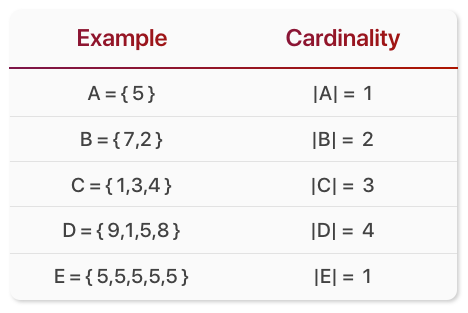
\includegraphics[width=300mm]{finitecardinality.png}
        \caption{Cardinalities of finite sets}
        \label{fig:enter-label}
        \end{figure}

        
        \item \textbf{Sets of interest}: Finite and infinite sets

        Finite sets have an integer cardinality but infinite sets are trickier

        \item \textbf{Examples of infinite sets}:
        Set of natural, prime, even, or odd #'s
        \item  \textbf{Cardinality of \textit{countable} infinite sets}: Sets that contain and infinite number of elements are denoted with (${\aleph}$)
        
        \item \textbf{Cardinality \textit{uncountable} infinite sets}: Uncountable infinite sets are denoted as (${\aleph}$) > (${\aleph}_{0}$)

        Uncountable infinite sets are sets that include irrational, rational or real numbers.

        

    \end{itemize}
    
  \end{block}

    \begin{block}{References}

    \nocite{*}
    \footnotesize
    \bibliographystyle{plain}
    \bibliography{poster}

  \end{block}


\end{column}

\separatorcolumn

\begin{column}{\colwidth}


  \begin{block}{How to compare the cardinality of infinite sets}

    \begin{figure}

    \begin{subfigure}
        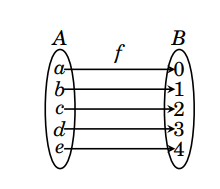
\includegraphics[width=0.3\textwidth,]{cardinalities.png}
        \caption{Cardinality}
        \end{subfigure}

    \begin{subfigure}
        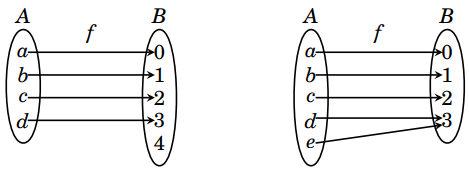
\includegraphics[width=0.7\textwidth]{nonequalcardinalities.png}
        \caption{Non-equal cardinalities}
    \end{subfigure}
    \end{figure}

  \end{block}


  \begin{block}{Cantor's diagonal argument}
    
    Cantor’s diagonal argument proves that there are more real numbers than integers
    
    The proof goes as follows:
    \begin{enumerate}
        \item Imagine you have a list of all the numbers in between 0 and 1
        \item If you create a number using a diagonal of the list, this creates a new, different number
        \item Since the number is unique, this proves the list is incomplete
    \end{enumerate}
    \begin{figure}
        \centering
        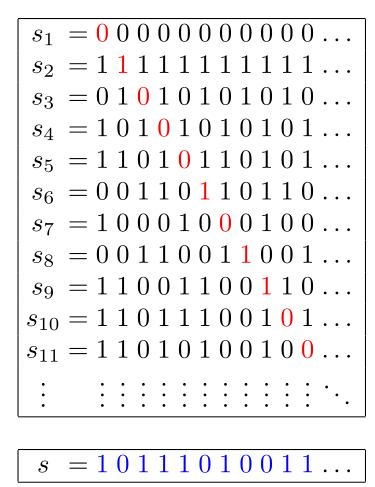
\includegraphics[width=0.6 \textwidth]{diagonal.png}
        \caption{Illustration of Cantor's Diagonal Argument}
        \label{fig:enter-label}
    \end{figure}

  \end{block}

  
\end{column}

\separatorcolumn

\begin{column}{\colwidth}

  \begin{exampleblock}{Hilbert's Infinite Hotel Paradox}


    Assume there's a hotel called the 'Infinite Hotel' where there is a countably infinite number of occupied rooms. The rooms correspond to the natural numbers in the number series.
    
    A guest needs a room so the manager would shift each guest to the immediate next room $n+1$,  so that room one is empty and the guest can be accommodated. This would work for any finite number of guests and rooms. 

\begin{figure}
    \centering
    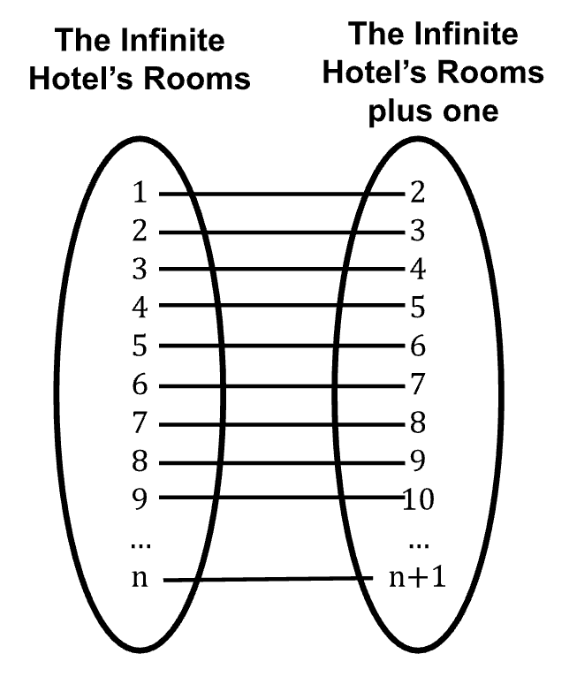
\includegraphics[width=0.4\linewidth]{hilberthotel_n+1.png}
    \caption{One-to-one correspondence of $n$ and $n+1$ to resemble countable infinities}
    \label{fig:enter-label}
\end{figure}

    \heading{Case 1: A Bus Arrives with an Infinite Number of Passengers Seeking Rooms}

    The manager would shift each guest to every other room, $2n$, so that it leaves the manager with an infinite odd number of empty rooms where the passengers could be accommodated.
    \begin{figure}
        \centering
        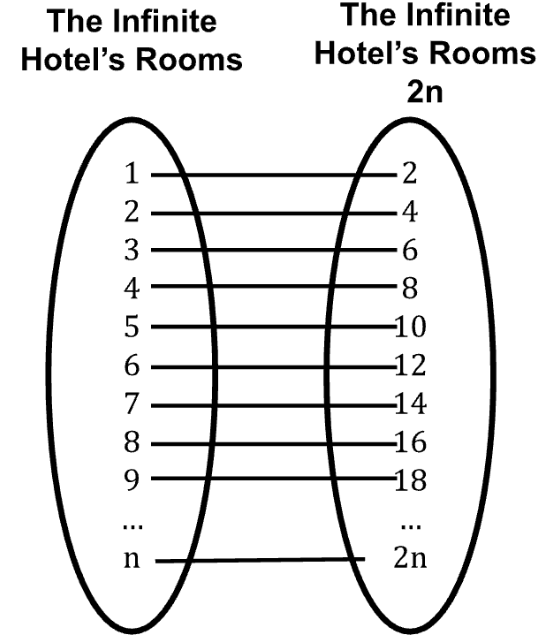
\includegraphics[width=0.4\linewidth]{hilberthotel_2n.png}
        \caption{One-to-one correspondence of $n$ and $n^2$ to resemble countable infinities}
        \label{fig:enter-label}
    \end{figure}

    \heading{Case 2: An Infinite Number of Buses Arrive with an Infinite Number of Passengers Seeking Rooms}

    The manager would shift each guest by the base of a prime number to the power of their room number. He starts with base $2$, moves to base $3$, moves to base $5$, and so on. This is because the set of all prime numbers $(2,3,5,7,11,...)$ is countably infinite.
\begin{figure}
    \centering
    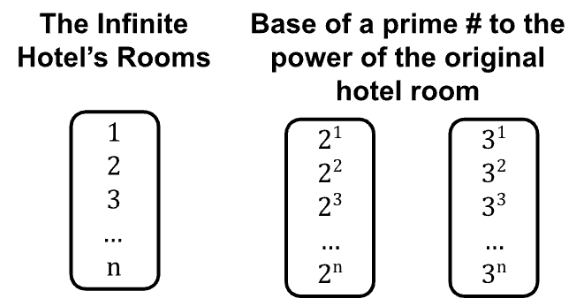
\includegraphics[width=0.45\linewidth]{hilberthotelprime#.png}
    \caption{The individual being moved by a prime number to the power of their room number}
    \label{fig:enter-label}
\end{figure}
  \end{exampleblock}

\end{column}

\separatorcolumn
\end{columns}
\end{frame}
\end{document}
